% Document Preamble
\documentclass[aspectratio=169]{beamer}
\usetheme{metropolis}
%\usepackage{color}
\usepackage{blowup}
\blowUp{target=x3}

\title{GE Silicone Sealants $^{222}$Rn Emanation Measurement}
\author[H. R. Glayzer]{H. Ryott Glayzer}
\institute[SDSMT]
{Lab Assistant\\
    SD Mines}
\date[2023]{December 2023}
\logo{
\includegraphics[height=1cm]{assets/SD_Mines_Logo.png}}

\begin{document}

\frame{\titlepage}

\begin{frame}{Sample Photos}
    \begin{figure}
        \centering
        
\includegraphics[width=0.4\textwidth]{assets/missing.jpg}
        \caption{photo not yet available}
    \end{figure}
\end{frame}

\begin{frame}{Overview of Emanation}
    \begin{itemize}
        \item Two samples were emanated throughout the latter half of 2023
        \begin{itemize}
            \item GE All-Purpose Silicone Sealant was emanated four times\\
                with a total of 465 hours of usable assay data.
            \item GE Advandced Silicone Sealant was emanated three times\\
                with a total of N hours of usable assay data.
        \end{itemize}
    \end{itemize}
\end{frame}

\begin{frame}{Rate vs. Time, Run 717}
    \begin{figure}
        \begin{center}
            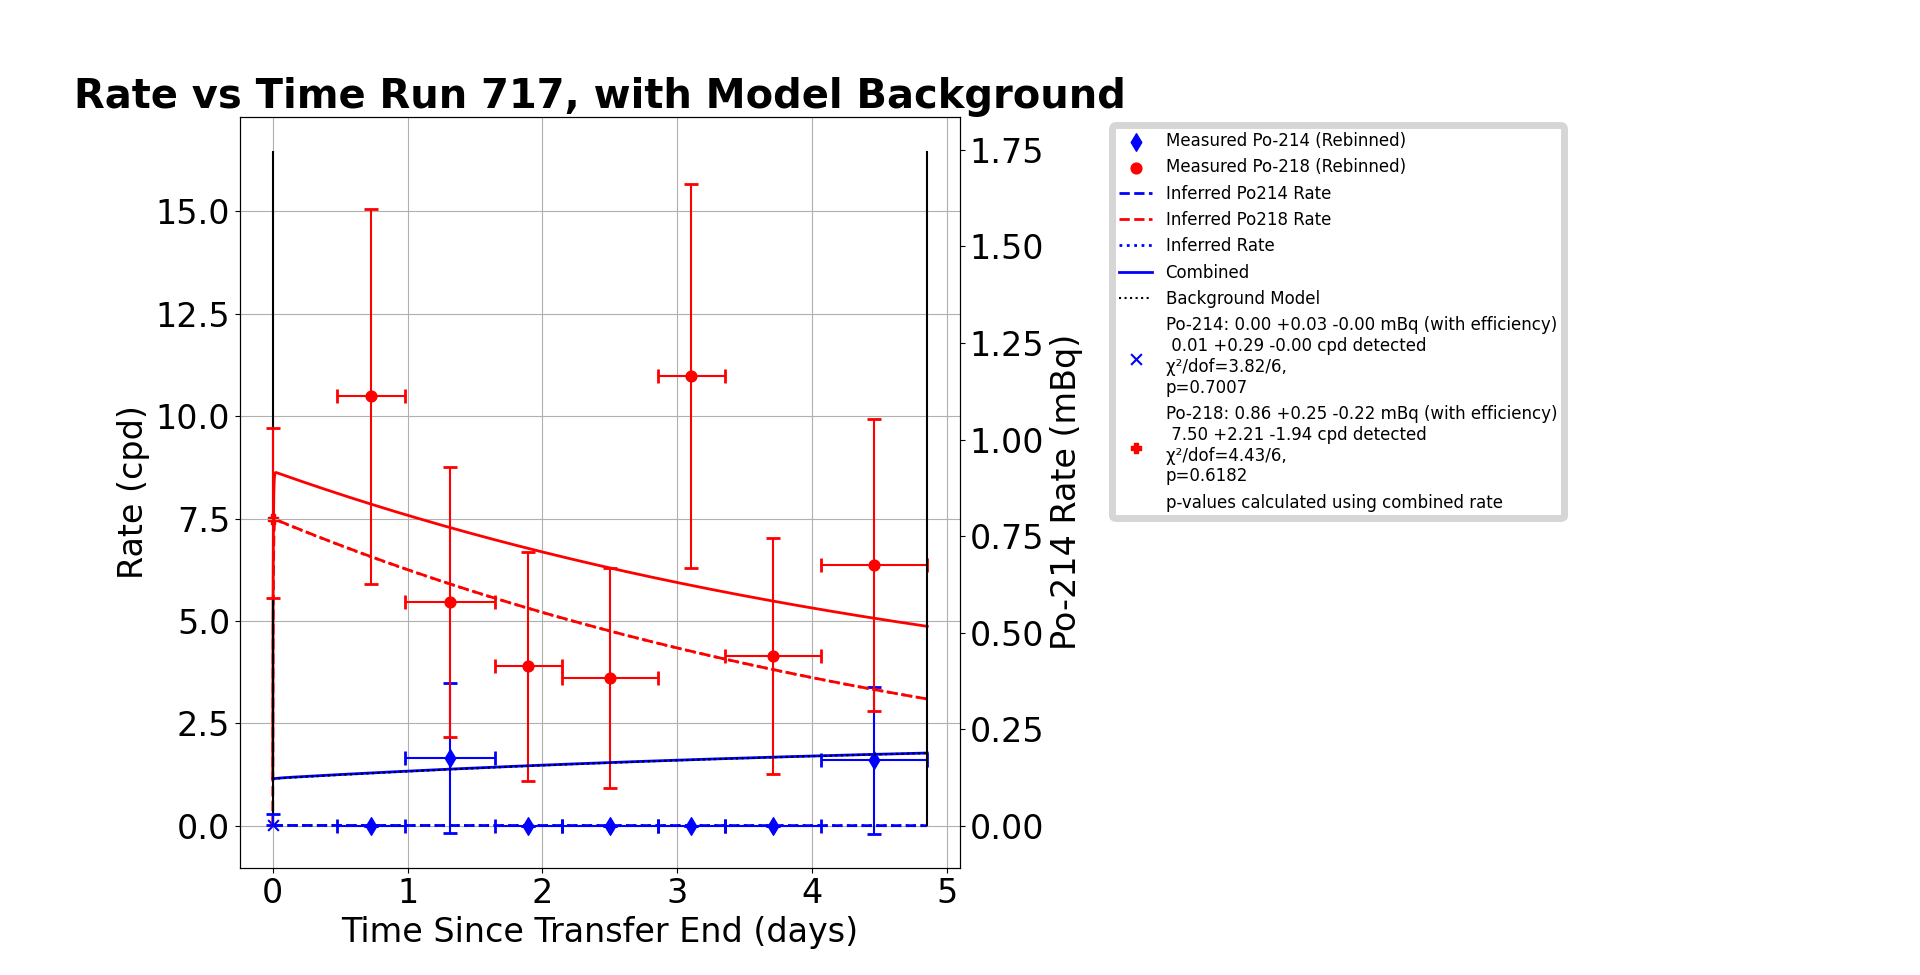
\includegraphics[width=0.9\textwidth]
            {assets/RvT_717.png}
            \caption{$^{222}$Rn Emanation Rate: 
            \textbf{0.00$^{+0.03}_{-0.00}$ mBq} (from $^{214}$Po Rate)}
        \end{center}
    \end{figure}  
\end{frame}

\begin{frame}{Run 717 Analysis}
    \begin{itemize}
        \item Emanation Rate was determined to be 0.00 $\pm$ 0.03 mBq.
        \item This determination was based on the observed emanation rate of $^{214}$Po.
        \item The $^{218}$Po rate wasn't used as poor resolution between the peaks of \@
            $^{218}$Po and $^{210}$Po likely caused $^{210}$Po events to spill over \@
            into the $^{218}$Po ROI
    \end{itemize}
\end{frame}

\begin{frame}{Rate vs. Time, Run 720}
    \begin{figure}
        \begin{center}
            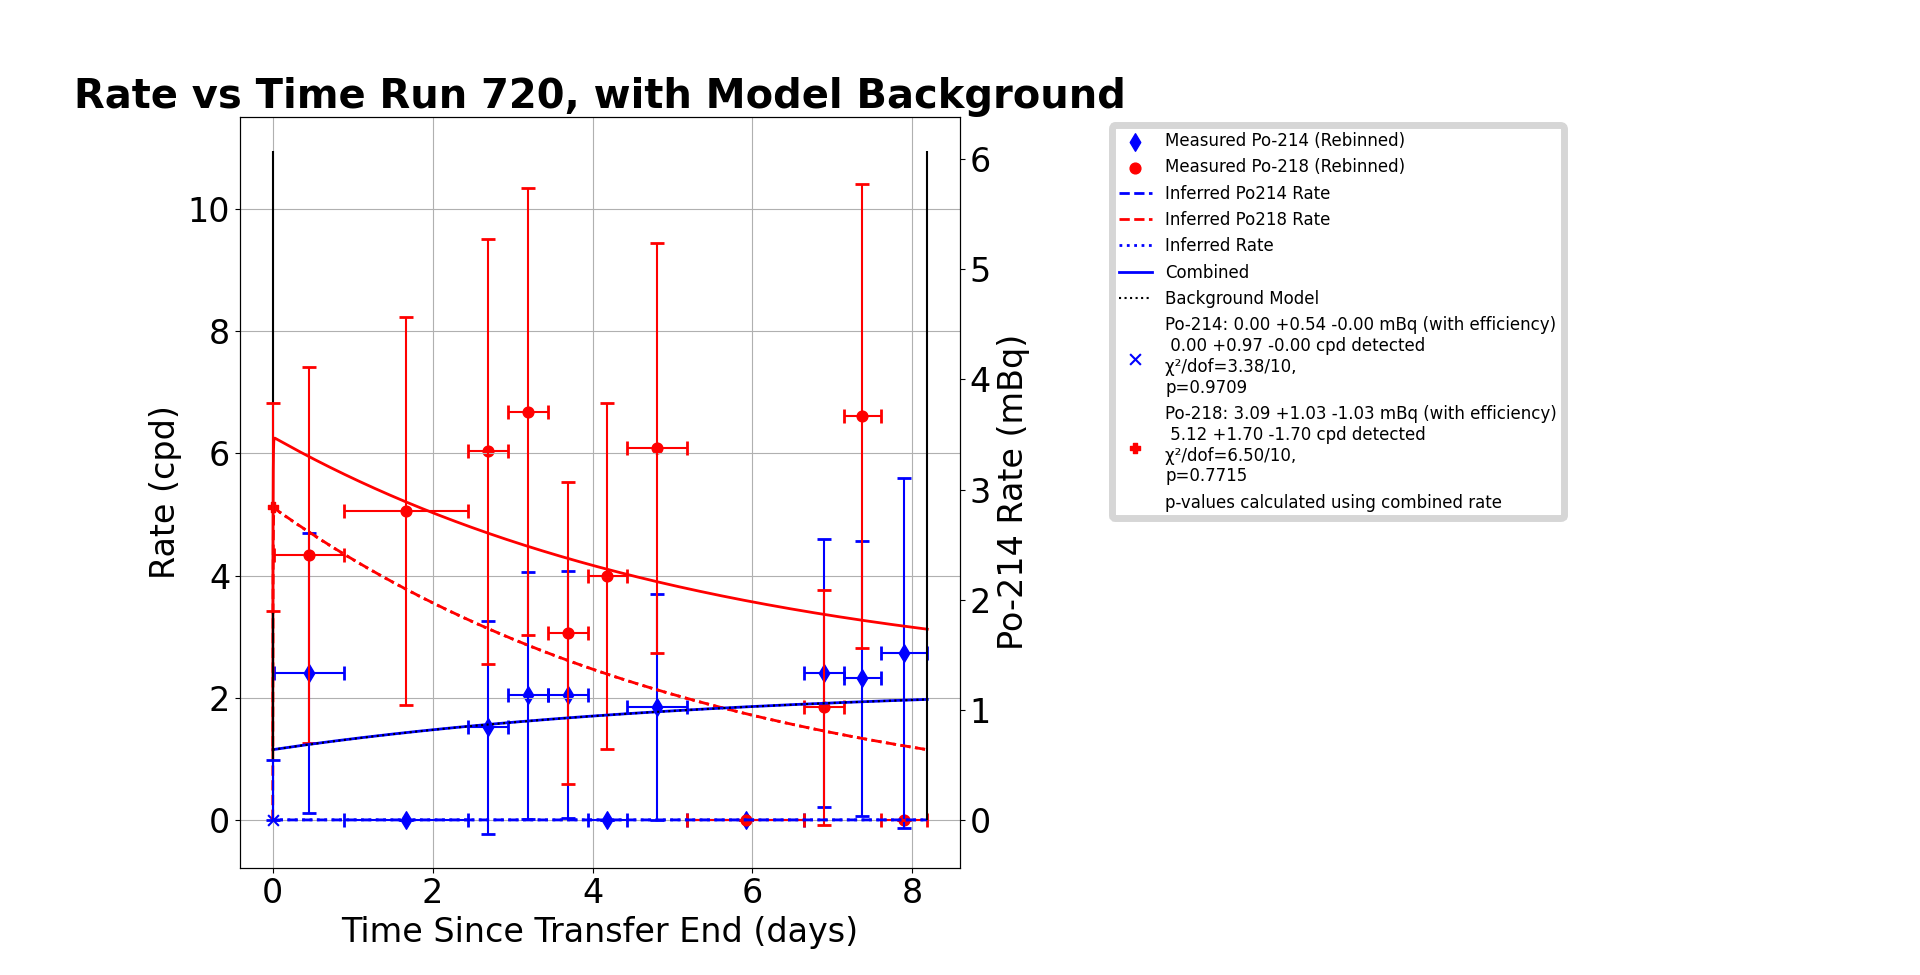
\includegraphics[width=0.9\textwidth]
            {assets/RvT_720.png}
            \caption{$^{222}$Rn Emanation Rate: 
            \textbf{0.00$^{+0.54}_{-0.00}$ mBq} (from $^{214}$Po rate)}
        \end{center}
    \end{figure}    
\end{frame}

\begin{frame}{Run 720 Analysis}
    \begin{itemize}
        \item Emanation Rate was determined to be \textbf{0.00 $^{+0.54}_{-0.00}$ mBq}.
        \item This determination was based on the observed emanation rate of $^{214}$Po.
        \item The $^{218}$Po rate wasn't used as poor resolution between the peaks of \@
            $^{218}$Po and $^{210}$Po likely caused $^{210}$Po events to spill over \@
            into the $^{218}$Po ROI
    \end{itemize}
\end{frame}

\begin{frame}{Rate vs. Time, Run 721}
    \begin{figure}
        \begin{center}
            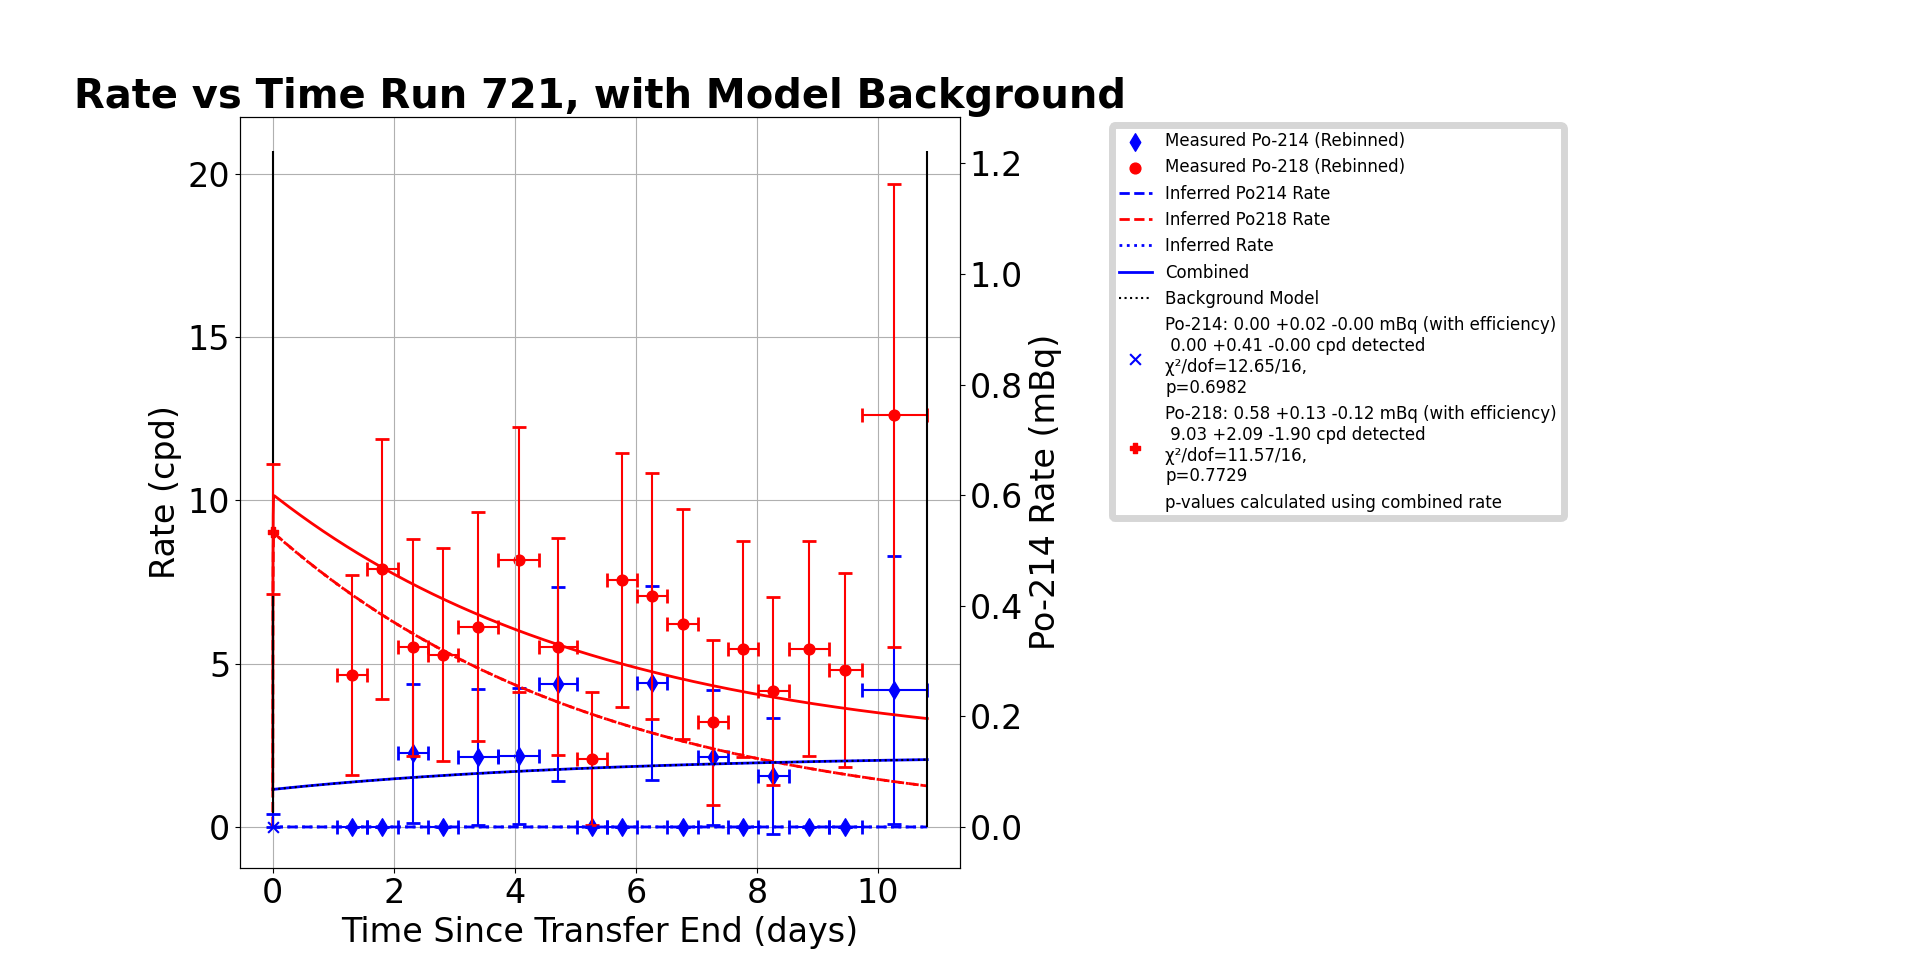
\includegraphics[width=0.9\textwidth]
            {assets/RvT_721.png}
            \caption{$^{222}$Rn Emanation Rate: 
            \textbf{0.00$^{+0.02}_{-0.00}$ mBq} (from $^{214}$Po rate)}
        \end{center}
    \end{figure}    
\end{frame}

\begin{frame}{Run 721 Analysis}
    \begin{itemize}
        \item Emanation Rate was determined to be \textbf{0.00 $^{+0.02}_{-0.00}$ mBq}.
        \item This determination was based on the observed emanation rate of $^{214}$Po.
        \item The $^{218}$Po rate wasn't used as poor resolution between the peaks of \@
            $^{218}$Po and $^{210}$Po likely caused $^{210}$Po events to spill over \@
            into the $^{218}$Po ROI
    \end{itemize}
\end{frame}

\begin{frame}{Rate vs. Time, Run 722}
    \begin{figure}
        \begin{center}
            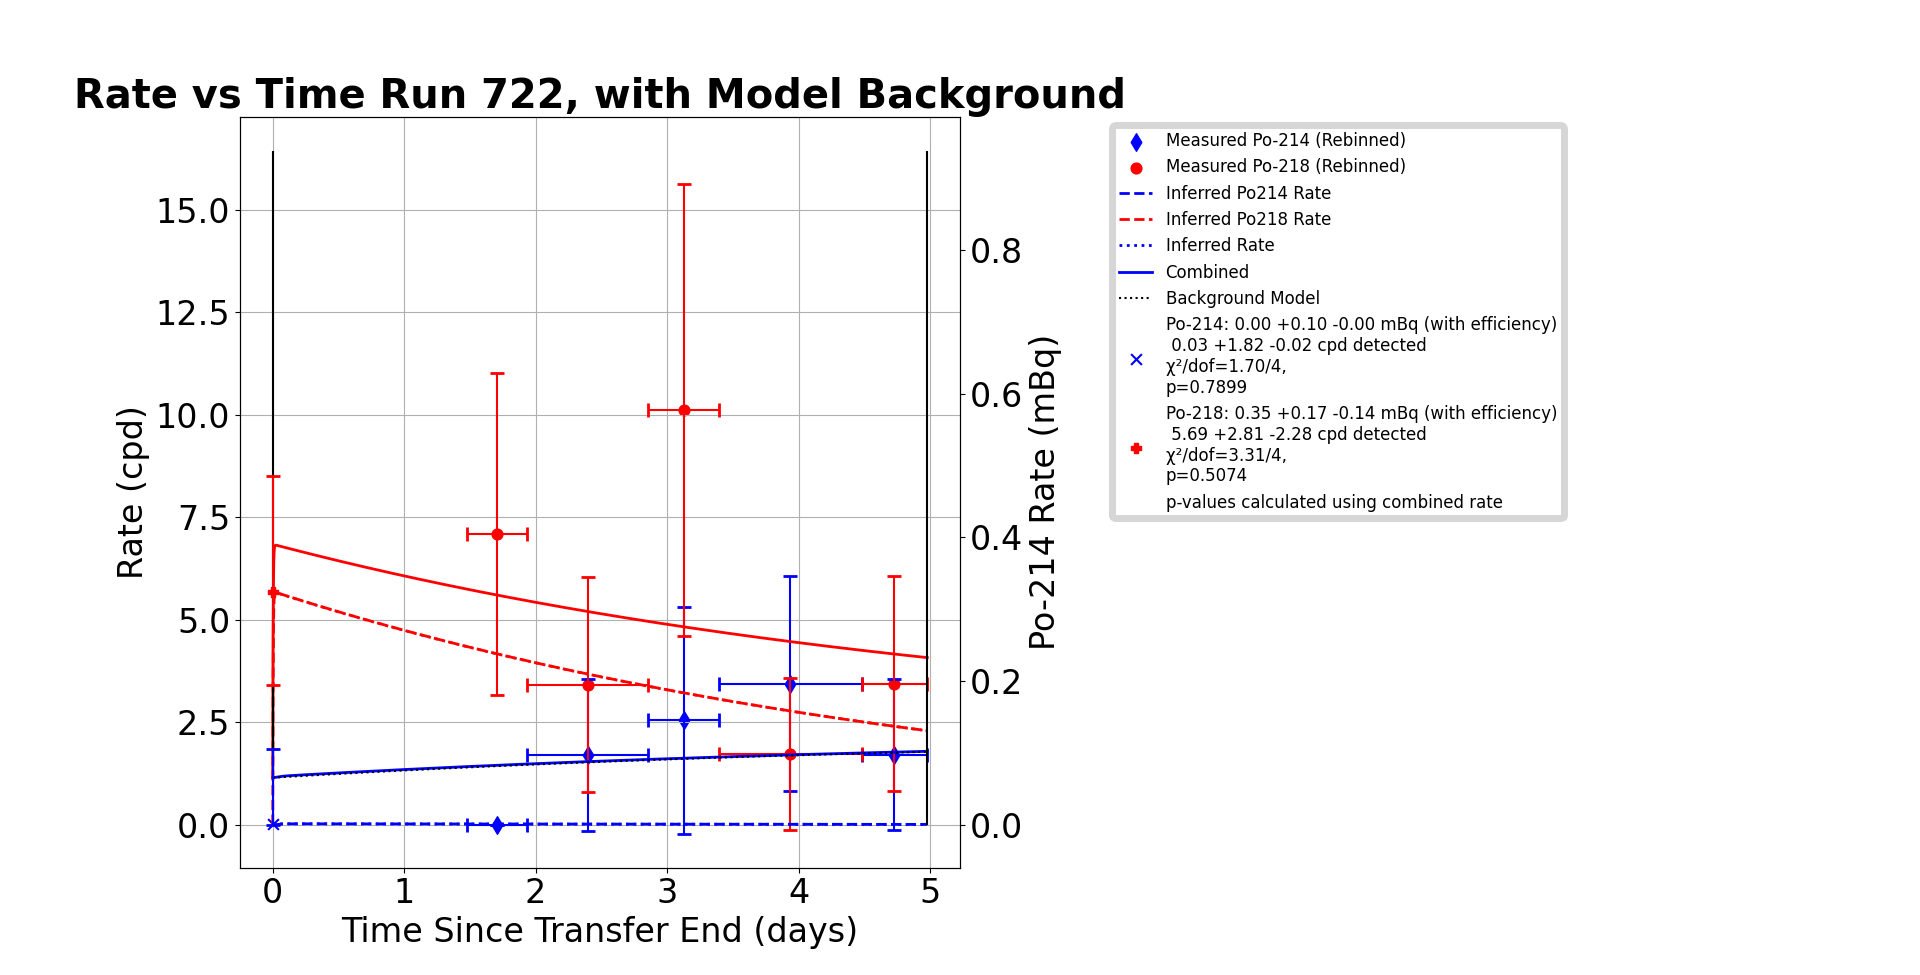
\includegraphics[width=0.9\textwidth]
            {assets/RvT_722.png}
            \caption{$^{222}$Rn Emanation Rate: 
            \textbf{0.00$^{+0.10}_{-0.00}$ mBq} (from $^{214}$Po rate)}
        \end{center}
    \end{figure}    
\end{frame}

\begin{frame}{Run 722 Analysis}
    \begin{itemize}
        \item Emanation Rate was determined to be \textbf{0.00 $^{+0.10}_{-0.00}$ mBq}.
        \item This determination was based on the observed emanation rate of $^{214}$Po.
        \item The $^{218}$Po rate wasn't used as poor resolution between the peaks of \@
            $^{218}$Po and $^{210}$Po likely caused $^{210}$Po events to spill over \@
            into the $^{218}$Po ROI
    \end{itemize}
\end{frame}

\begin{frame}{Backup Slides}
    Backup Slides contain additional data and information that may be helpful
    to provide context if questions come up.
\end{frame}




\end{document}
